\chapter{Краткий обзор общеизвестных структур данных}
\label{short-visit-to-common-data-structures}
\section{Обзор недолгий, обещаю!}
\label{wont-be-too-long-promised}
Функциональное подмножество Erlang вы, скорее всего, теперь понимаете достаточно неплохо, и текст многих программ смогли бы читать без проблем.
Но, тем не менее, готов поспорить, что вам не вполне ясно как построить настоящую полезную программу, хоть последняя глава и рассказывала о том, как решать задачи в функциональном стиле.
Говорю я об этом потому, что испытывал точно такие же чувства приблизительно в этот же момент моего обучения.
Впрочем, если у вас такой проблемы нет, то поздравляю!

В любом случае, я исхожу из того, что мы рассмотрели много всего: большинство базовых типов данных, оболочку, то как писать модули и функции (с рекурсией), различные способы компиляции, управление логикой программы, перехват исключений, абстракция некоторых общих операций и т.д.
Также мы познакомились с хранением данных в кортежах, списках, и рассмотрели незаконченную реализацию двоичного дерева поиска.
Но мы совсем не рассматривали другие структуры данных, которые предоставляет программисту стандартная библиотека Erlang.
\section{Записи}
\label{records}
\begin{wrapfigure}{r}{0.2\linewidth}
    
\includegraphics[width=1\linewidth]{record-player.png}
\end{wrapfigure}
Прежде всего, записи \--- это хак.
Они \--- что\--то вроде запоздалой мысли, пришедшей в голову разработчикам языка, и поэтому имеют свои недостатки.
О недостатках я расскажу позже.
Записи очень пригождаются, если нам нужна небольшая структура данных, которая предоставляет прямой доступ к именованным атрибутам.
Поэтому записи в Erlang очень похожи на структуры в C (если вы знакомы с языком C).

Они объявляются так же как и атрибуты модуля:
\begin{lstlisting}[style=erlang]
-module(records).
-compile(export_all).
 
 -record(robot, {name,
                 type=industrial,
                 hobbies,
                 details=[]}).
\end{lstlisting}

Эта запись представляет информацию о роботе и имеет 4 поля: имя, тип робота, его хобби и подробности.
Для полей, хранящих тип и подробности, кроме того, задано значение по умолчанию: соответственно \ops{industrial} и \ops{[]}.
Вот так в модуле \href{http://learnyousomeerlang.com/static/erlang/records.erl}{records} можно объявить запись:
\begin{lstlisting}[style=erlang]
first_robot() ->
    #robot{name="Mechatron",
        type=handmade,
        details=["Moved by a small man inside"]}.
\end{lstlisting}

Запускаем код:
\begin{lstlisting}[style=erlang]
1> c(records).
{ok,records}
2> records:first_robot().
{robot,"Mechatron",handmade,undefined,
    ["Moved by a small man inside"]}
\end{lstlisting}

Опа!
Вот и хак!
Записи в Erlang \--- всего лишь синтаксический сахар поверх кортежей.
К счастью, ситуацию можно улучшить.
В оболочке Erlang есть команда \ops{rr(Module)}, которая позволяет загружать определения записей из \emph{Module}:
\begin{lstlisting}[style=erlang]
3> rr(records).
[robot]
4> records:first_robot().        
#robot{name = "Mechatron",type = handmade,
    hobbies = undefined,
    details = ["Moved by a small man inside"]}
\end{lstlisting}

Совсем другое дело!
Так с записями намного легче работать.
Вы можете заметить, что в \ops{first\_robot/0} мы не определяли поле \ops{hobbies}, и в его определении не было значения по умолчанию.
Erlang неявно присваивает неинициализированным полям значение undefined.

Следующая функция поможет нам увидеть, как ведут себя значения по умолчанию, установленные в определении записи \ops{robot}:
\begin{lstlisting}[style=erlang]
car_factory(CorpName) ->
    #robot{name=CorpName, hobbies="building cars"}.
\end{lstlisting}

И запускаем:
\begin{lstlisting}[style=erlang]
5> c(records).
{ok,records}
6> records:car_factory("Jokeswagen").
#robot{name = "Jokeswagen",type = industrial,
    hobbies = "building cars",details = []}
\end{lstlisting}

Теперь у нас есть промышленный робот, который любит заниматься постройкой машин.\\
\colorbox{lgray}
{
\begin{minipage}{1.0\linewidth}
    \textbf{Замечание:}  функция \ops{rr()} может принимать не только имя модуля, но и шаблоны (вида \ops{rr(''*'')}) и список загружаемых записей вторым аргументом.

    В оболочке есть ещё несколько функций, с помощью которых можно манипулировать записями: \ops{rd(Name, Definition)} позволяет определять запись способом похожим на \ops{-record(Name, Definition)}, который мы использовали в нашем модуле.
    Команду \ops{rf()} можно использовать для <<выгрузки>> всех записей, а \ops{rf(Name)} и \ops{rf([Names])} \--- чтобы избавиться только от указанных определений.

    Можно использовать команду \ops{rl()} для вывода определений всех записей в виде пригодном для непосредственного копирования в модуль, или её формы \ops{rl(Name)} и \ops{rl([Names])} для вывода лишь указанных записей.

    И, наконец, команда \ops{rp(Term)} конвертирует кортеж в запись (при условии, что запись определена).
\end{minipage}
}

Но на одних записях далеко не уедешь.
Нужно уметь извлекать из них значения.
Делается это двумя способами.
Первый \--- специальный <<синтаксис с точкой>>.
Представим, что определение записи о роботе уже загружено:
\begin{lstlisting}[style=erlang]
5> Crusher = #robot{name="Crusher", hobbies=["Crushing people","petting cats"]}.
#robot{name = "Crusher",type = industrial,
    hobbies = ["Crushing people","petting cats"],
    details = []}
6> Crusher#robot.hobbies.
["Crushing people","petting cats"]
\end{lstlisting}

Синтаксис красотой не блещет.
Он выглядит так потому, что записи по природе своей \--- кортежи.
Не более чем трюк компилятора.
Поэтому для записи приходится хранить ключевые слова, которые определяют, к какой переменной она относится. Именно поэтому \ops{\#robot} \--- часть \ops{Crusher\#robot.hobbies}.
Всё это, конечно, огорчает, но ничего не поделаешь.
Вложенные записи выглядят ещё уродливее:
\begin{lstlisting}[style=erlang]
7> NestedBot = #robot{details=#robot{name="erNest"}}.
#robot{name = undefined,type = industrial,
    hobbies = undefined,
    details = #robot{name = "erNest",type = industrial,
                    hobbies = undefined,details = []}}
8> (NestedBot#robot.details)#robot.name.
"erNest"
\end{lstlisting}

И да, скобки обязательны.\\
\colorbox{lgray}
{
\begin{minipage}{1.0\linewidth}
    \textbf{Дополнение:} \\ 
    Начиная с ревизии R14A появилась возможность записывать вложенные записи без скобок.
    Вышеприведённый пример \emph{NestedBot} можно также записать как \ops{NestedRobot\#robot.details\#robot.name}.
    Работать такая запись будет аналогично.
\end{minipage}
}

Рассмотрим следующий пример, чтобы глубже обозначить зависимость записей от кортежей:
\begin{lstlisting}[style=erlang]
9> #robot.type.
3
\end{lstlisting}

Код выводит номер элемента кортежа, который реализует данное поле.

У записей есть одна оправдывающая их особенность \--- записи можно использовать в заголовках функции для сопоставления с образцом, а также в охранных выражениях.
Определите в начале файла новую запись, и добавьте несколько функций:
\begin{lstlisting}[style=erlang]
-record(user, {id, name, group, age}).
 
%% use pattern matching to filter
admin_panel(#user{name=Name, group=admin}) ->
    Name ++ " is allowed!";
admin_panel(#user{name=Name}) ->
    Name ++ " is not allowed".
 
%% can extend user without problem
adult_section(U = #user{}) when U#user.age >= 18 ->
    %% Show stuff that can't be written in such a text
    allowed;
adult_section(_) ->
    %% redirect to sesame street site
    forbidden.
\end{lstlisting}

В функции \ops{admin\_panel/1} показан синтаксис, который позволяет связывать переменную с любым полем записи (можно связывать переменные сразу с несколькими полями).
Следует отметить, что для связывания целой записи с переменной в функции \ops{adult\_section/1}, необходимо выполнить код \ops{SomeVar = \#some\_record\{\}}.
И, как обычно, скомпилировать:
\begin{lstlisting}[style=erlang]
10> c(records).
{ok,records}
11> rr(records).
[robot,user]
12> records:admin_panel(#user{id=1, name="ferd", group=admin, age=96}).
"ferd is allowed!"
13> records:admin_panel(#user{id=2, name="you", group=users, age=66}).
"you is not allowed"
14> records:adult_section(#user{id=21, name="Bill", group=users, age=72}).
allowed
15> records:adult_section(#user{id=22, name="Noah", group=users, age=13}).
forbidden
\end{lstlisting}

На этом примере можно увидеть, что нет необходимости делать сопоставление по всем элементам кортежа, или вообще иметь во время написания функции представление о количестве этих элементов.
Можно провести сопоставление только по возрасту или группе, а об остальных полях даже и не вспоминать.
Если бы нам пришлось использовать обычный кортеж, то определение функции выглядело бы приблизительно так: \ops{function(\{record, \_, \_, ICareAboutThis, \_, \_\}) -> \ldots}.
Как только кто\--либо решит добавить в кортеж новый элемент, кто\--то другой (скорее всего весьма недовольный этой ситуацией) будет обязан исправить все функции, в которых используется этот кортеж.

Эта функция демонстрирует как можно обновлять записи (иначе пользы от них было бы мало):
\begin{lstlisting}[style=erlang]
repairman(Rob) ->
    Details = Rob#robot.details,
    NewRob = Rob#robot{details=["Repaired by repairman"|Details]},
    {repaired, NewRob}.
\end{lstlisting}

А затем:
\begin{lstlisting}[style=erlang]
16> c(records).
{ok,records}
17> records:repairman(#robot{name="Ulbert", hobbies=["trying to have feelings"]}).
{repaired,#robot{name = "Ulbert",type = industrial,
    hobbies = ["trying to have feelings"],
    details = ["Repaired by repairman"]}}
\end{lstlisting}

Как видите, моего робота починили.
Здесь для обновления записей используется особенный синтаксис.
Может показаться, что мы обновляем ту же самую запись (\ops{Rob\#robot\{Field=NewValue\}}), но на самом деле это просто уловки компилятора, которые маскируют скрытый вызов функции \ops{\href{http://erldocs.com/R15B/erts/erlang.html\#setelement/3}{erlang:setelement/3}}.

И в заключение хотелось бы сказать, что записи весьма полезны, а дублирование кода не очень.
Поэтому программисты на Erlang часто совмещают использование одних и тех же записей в нескольких модулях при помощи \emph{заголовочных файлов}.
Файл заголовков в Erlang очень похож на их аналог в языке C.
Это просто фрагмент кода, который добавляется в модуль, как будто он там был всегда.
Создайте файл \href{http://learnyousomeerlang.com/static/erlang/records.hrl}{records.hrl} и добавьте в него следующий код:
\begin{lstlisting}[style=erlang]
%% this is a .hrl (header) file.
-record(included, {some_field,
                  some_default = "yeah!",
                  unimaginative_name}).
\end{lstlisting}

Чтобы включить этот заголовок в \href{http://learnyousomeerlang.com/static/erlang/records.erl}{records.erl}, нужно просто добавить в модуль такую строчку:
\begin{lstlisting}[style=erlang,]
-include("records.hrl").
\end{lstlisting}

И в следующей функции применить запись:
\begin{lstlisting}[style=erlang]
included() -> #included{some_field="Some value"}.
\end{lstlisting}

А теперь, как обычно, проверим:
\begin{lstlisting}[style=erlang]
18> c(records).
{ok,records}
19> rr(records).
[included,robot,user]
20> records:included().
#included{some_field = "Some value",some_default = "yeah!",
         unimaginative_name = undefined}
\end{lstlisting}

Ура!
Довольно о записях.
Приятными их, конечно, не назовёшь, но они полезны.
У них некрасивый синтаксис, они реализованы при помощи хака, но, тем не менее, они играют достаточно важную роль в удобстве поддержки вашего кода.\\
\colorbox{lgray}
{
\begin{minipage}{1.0\linewidth}
    \textbf{Замечание:} в проектах с открытым кодом вы сможете часто встретить описанный здесь метод.
В проект добавляется \ops{.hrl} файл, содержащий записи, которые используются во всех модулях приложения.
Хоть я и считаю, что обязан задокументировать этот способ использования записей, но я настоятельно рекомендую применять только локальные определения, которые действуют в пределах одного модуля.
Если вам нужно, чтобы какой\--либо другой модуль имел доступ к внутренему устройству записи \--- напишите несколько функций, которые предоставляют доступ к полям, а подробности реализации сделайте как можно более закрытыми.
Это правило позволяет предотвратить конфликт имён, помогает избежать проблем с обновлением кода, улучшает его общую читаемость и упрощает поддержку.
\end{minipage}
}
\section{Хранилища пар ключ\--значение}
\label{key-value-stores}
Несколько глав назад вы построили дерево и собирались его использовать в качестве хранилища пар ключ\--значение для адресной книги.
Книга получилась хреновая: удалять значения из неё мы не могли, да и найти ей достойное применение тоже не получилось.
С её помощью нам удалось хорошо продемонстрировать принцип работы рекурсии, но не более.
Пришло время познакомить вас с несколькими полезными структурами, предназначение которых \--- хранение данных, связанных с определённым ключом.
Я не буду рассказывать подробно о каждой функции или делать полный обзор модулей.
Я просто дам вам ссылку на документацию.
Считайте, что моей обязанностью является <<улучшение осведомлённости о хранилищах пар ключ\--значение в Erlang>> или что\--то вроде того.
Ну а что, звание звучит неплохо.
Осталось только нашивку сделать.
\begin{wrapfigure}{r}{0.2\linewidth}
    
\includegraphics[width=1\linewidth]{key.png}
\end{wrapfigure}

Для хранения небольших объёмов данных можно использовать два вида структур.
Первая называется \emph{proplist} (список свойств).
Proplist \--- это любой список кортежей вида \ops{[\{Key, Value\}]}.
На этом правила, определяющие её устройство, заканчиваются.
Немного странная структура.
Список может также содержать булевы значения, целые числа и вообще всё что вам угодно.
Но сейчас нас интересует именно список, наполненный кортежами с ключом и значением.
Для работы с proplist\--ами можно использовать модуль \href{http://erldocs.com/R15B/stdlib/proplists.html}{proplists}.
Он содержит функции \ops{\href{http://erldocs.com/R15B/stdlib/proplists.html\#delete/2}{proplists:delete/2}}, \ops{\href{http://erldocs.com/R15B/stdlib/proplists.html\#get\_value/2}{proplists:get\_value/2}}, \ops{\href{http://erldocs.com/R15B/stdlib/proplists.html\#get\_all\_values/2}{proplists:get\_all\_values/2}}, \ops{\href{http://erldocs.com/R15B/stdlib/proplists.html\#lookup/2}{proplists:lookup/2}} и \ops{\href{http://erldocs.com/R15B/stdlib/proplists.html\#lookup\_all/2}{proplists:lookup\_all/2}}.

Вы заметите, что в этом списке нет функций для добавления и удаления элементов.
Это даёт представление о том, насколько нечётко определены proplist\--ы как структура данных.
Чтобы получить возможность добавлять и удалять элементы, придётся вручную добавлять их при помощи конструктора (\ops{[NewElement|OldList]}) и использовать, например, функцию \ops{\href{http://erldocs.com/R15B/stdlib/lists.html\#keyreplace/4}{lists:keyreplace/4}}.
Для работы с одной небольшой структурой данных приходится использовать два модуля, и это решение не назовёшь кристально чистым.
Но благодаря нечёткому определению proplist\--ов, их часто используют для представления списка настроек или общего описания какого\--либо предмета.
Proplist\--ы нельзя назвать полной структурой данных.
Их скорее можно отнести к общему шаблону, который используется для представления некоторого объекта или предмета при помощи списков и кортежей.
А модуль proplists \--- что\--то вроде инструментария поверх этого шаблона.

Если вам понадобилось хранилище пар ключ\--значение для небольших объёмов данных c более полной функциональностью, то модуль \href{http://erldocs.com/R15B/stdlib/orddict.html}{orddict} \--- это то что нужно.
Orddict\--ы (упорядоченные словари) \--- это proplist\--ы со склонностью к формализму.
Каждый ключ может присутствовать в структуре только один раз, список упорядочивается для ускорения поиска и т.д.
Обычные CRUD\--операции представлены функциями \ops{\href{http://erldocs.com/R15B/stdlib/orddict.html\#store/3}{orddict:store/3}}, \ops{\href{http://erldocs.com/R15B/stdlib/orddict.html\#find/2}{orddict:find/2}} (на случай, если вам точно не известно, есть ли такой ключ в словаре), \ops{\href{http://erldocs.com/R15B/stdlib/orddict.html\#fetch/2}{orddict:fetch/2}} (когда вы знаете, что такой ключ в словаре присутствует, или что он там \textbf{должен} быть) и \ops{\href{http://erldocs.com/R15B/stdlib/orddict.html\#erase/2}{orddict:erase/2}}.
\begin{wrapfigure}{l}{0.35\linewidth}
    
\includegraphics[width=1\linewidth]{dict.png}
\end{wrapfigure}

Orddict\--ы представляют собой неплохой компромисс между сложностью и эффективностью, при условии, что количество элементов приблизительно равно 75 (ознакомьтесь с \href{http://learnyousomeerlang.com/static/erlang/keyval\_benchmark.erl}{моими замерами}).
Если количество элементов превышает это число, то вам нужно переключиться на какое\--либо другое хранилище пар ключ\--значение.

В принципе, существует два модуля/структуры для работы с большими объёмами данных: \href{http://erldocs.com/R15B/stdlib/dict.html}{dicts} и \href{http://erldocs.com/R15B/stdlib/gb\_trees.html}{gb\_trees}.
У словарей такой же интерфейс как и у orddict\--ов: \ops{\href{http://erldocs.com/R15B/stdlib/dict.html\#store/3}{dict:store/3}}, \ops{\href{http://erldocs.com/R15B/stdlib/dict.html\#find/2}{dict:find/2}}, \ops{\href{http://erldocs.com/R15B/stdlib/dict.html\#fetch/2}{dict:fetch/2}}, \ops{\href{http://erldocs.com/R15B/stdlib/dict.html\#erase/2}{dict:erase/2}} и любая другая функция, например \ops{\href{http://erldocs.com/R15B/stdlib/dict.html\#map/2}{dict:map/2}} и \ops{\href{http://erldocs.com/R15B/stdlib/dict.html\#fold/2}{dict:fold/2}} (их очень удобно использовать при работе со всей структурой).
Так что если вам нужно расширить orddict \--- словари очень хорошо справятся с этой задачей.

Зато у сбалансированных деревьев общего назначения есть несколько функций, которые предоставляют прямой доступ к управлению структурой.
По сути, у gb\_trees есть два режима: в первом режиме вам известно о структуре всё (я называю этот режим <<умным (smart) режимом>>), и второй, в котором вы не можете делать какие\--либо предположения о структуре (я называю этот режим <<наивным (naive) режимом>>).
В наивном режиме доступны функции \ops{\href{http://erldocs.com/R15B/stdlib/gb\_trees.html\#enter/2}{gb\_trees:enter/2}}, \ops{\href{http://erldocs.com/R15B/stdlib/gb\_trees.html\#lookup/2}{gb\_trees:lookup/2}} и \ops{\href{http://erldocs.com/R15B/stdlib/gb\_trees.html\#delete\_any/2}{gb\_trees:delete\_any/2}}.
В умном режиме им соответствуют функции \ops{\href{http://erldocs.com/R15B/stdlib/gb\_trees.html\#insert/3}{gb\_trees:insert/3}}, \ops{\href{http://erldocs.com/R15B/stdlib/gb\_trees.html\#get/2}{gb\_trees:get/2}}, \ops{\href{http://erldocs.com/R15B/stdlib/gb\_trees.html\#update/3}{gb\_trees:update/3}} и \ops{\href{http://erldocs.com/R15B/stdlib/gb\_trees.html\#delete/2}{gb\_trees:delete/2}}.
Ещё можно использовать \ops{\href{http://erldocs.com/R15B/stdlib/gb\_trees.html\#map/2}{gb\_trees:map/2}}, а такая возможность никогда не бывает лишней.

Недостатком <<наивных>> функций, в сравнении с <<умными>>, является то, что после вставки нового элемента (или удаления нескольких), может появиться необходимость перебалансировки дерева.
Это отнимет какое\--то время и потребует некоторого количества памяти (даже если просто нужно будет убедиться в том, что перебалансировка не нужна).
Все <<умные>> функции предполагают, что искомый ключ присутствует в дереве.
Это позволяет пропустить все проверки и уменьшает время исполнения операций.

Когда же всё\--таки необходимо использовать gb\_trees вместо dict?
Решение не вполне очевидно.
Результаты исполнения моего \href{http://learnyousomeerlang.com/static/erlang/keyval\_benchmark.erl}{измерительного модуля}, свидетельствуют о том, что gb\_trees и dicts показывают во многих случаях приблизительно одинаковый результат.
Но измерения также говорят о том, что dicts показывает самую высокую скорость при считывании значений, а gb\_trees отрабатывает немного быстрее в других операциях.
Вы cможете делать выбор, отталкиваясь от того, какие операции для вашей задачи важнее других.

Да, ещё запомните, что у dicts есть функция свёртки (fold), а у gb\_trees \--- нет.
Вместо неё у gb\_trees есть функция\--\emph{итератор}, которая возвращает часть дерева, к которой можно применить вызов \ops{gb\_trees:next(Iterator)} и получить следующее по порядку значение.
Так что к структуре gb\_trees не получится применять универсальный fold, а придётся писать собственные рекурсивные функции.
Зато gb\_trees предоставляет быстрый доступ к наименьшему и наибольшему элементу в структуре при помощи функций \ops{\href{http://erldocs.com/R15B/stdlib/gb\_trees.html\#smallest/1}{gb\_trees:smallest/1}} и \ops{\href{http://erldocs.com/R15B/stdlib/gb\_trees.html\#largest/1}{gb\_trees:largest/1}}.

Можно сказать, что при выборе хранилища пар ключ\--значение, вы должны руководствоваться нуждами вашего приложения.
На ваше решение могут оказать влияние различные факторы, каждый из которых по\--своему важен: сколько данных вам необходимо хранить, какие операции с этими данными нужно выполнять и прочее.
Чтобы убедиться в правильности вашего выбора, проводите измерения, профилируйте код, сравнивайте скорость исполнения.\\
\colorbox{lgray}
{
\begin{minipage}{1.0\linewidth}
    \textbf{Замечание:} существуют специальные хранилища пар ключ\--значение для работы с ресурсами различного размера.
    Это \href{http://erldocs.com/R15B/stdlib/ets.html}{ETS таблицы}, \href{http://erldocs.com/R15B/stdlib/dets.html}{DETS таблицы} и база данных \href{http://erldocs.com/R15B/mnesia/mnesia.html?search=mnesia&i=0}{mnesia}.
    Но так как их использование тесно связано с концепцией множественных процессов и распределённостью, мы затронем их позже.
    Я оставляю эту информацию как ориентир, призванный разжечь ваше любопытство и направить заинтересовавшихся в нужном направлении.
\end{minipage}
}
\section{Массивы}
\label{arrays}
А как быть с кодом, для которого нужны структуры данных, принимающие только числовые данные?
В нём можно использовать \href{http://erldocs.com/R15B/stdlib/array.html}{массивы}.
К их элементам можно обращаться при помощи числовой идексации, а также применять ко всей структуре операцию свёртки.
При этом есть возможность игнорировать позиции с неопределённым значением.
\colorbox{lorange}
{
    \begin{minipage}{1.0\linewidth}
        \textbf{Не забывайтесь:}\\
В противоположность своим императивным собратьям, массивы Erlang не могут выполнять операции вставки и поиска за константное время.
На практике массивы используют редко, так как они обычно медленнее массивов в языках, подерживающих деструктивное присваивание, и стиль программирования на Erlang не очень хорошо стыкуется с массивами и матрицами.\\
В задачах, где необходимо использовать матричные манипуляции и массивы, программисты склоняются к использованию концепции, которая называется \href{http://www.erlang.org/doc/tutorial/c\_port.html}{Ports}.
С её помощью исполнение тяжёлых операций перекладывается на другие языки.
К той же концепции можно отнести \href{http://www.erlang.org/doc/tutorial/cnode.html}{C-Nodes}, \href{http://www.erlang.org/doc/tutorial/c\_portdriver.html}{Linked in drivers} и \href{http://erldocs.com/R15B/erts/erl\_nif.html}{NIF} (экспериментальная поддержка в R13B03+).\\
Ещё одна странность массивов заключается в том, что их индексация начинается с 0 (в противоположность кортежам или спискам).
Такая же индексация используется и в \href{http://erldocs.com/R15B/stdlib/re.html}{модуле для работы с регулярными выражениями}.
Будьте внимательны.
    \end{minipage}
}
\section{Набор наборов}
\label{a-set-of-sets}
\begin{wrapfigure}{r}{0.38\linewidth}
    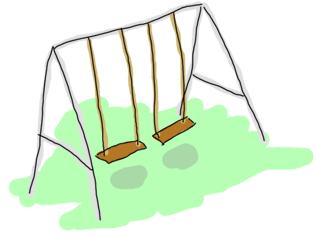
\includegraphics[width=1\linewidth]{swingset.png}
\end{wrapfigure}
Если вам когда\--либо приходилось изучать теорию множеств, то у вас есть представление о свойствах наборов.
Если не приходилось, то вы, возможно, не захотите читать дальше.
Но я всё\--таки скажу, что наборы \--- это группы уникальных элементов, которые можно сравнивать.
Над ними также можно совершать  различные действия: найти элементы, которые одновременно принадлежат двум группам, или не принадлежат ни одной группе, или принадлежат лишь одной из групп и т.д.
Можно также производить более сложные операции, которые позволяют определить связи между группами, совершать над ними действия, и ещё много всего.
Не буду погружаться в теорию (опять же, она выходит за рамки этой книги), а просто опишу наборы такими, как есть.

В Erlang существует 4 основных модуля, предназначенных для работы с наборами.
Сперва такое обилие может показаться странным, но оно порождено единым мнением разработчиков, что <<лучшего>> способа реализации наборов не существует.
Вот эти четыре модуля: \href{http://erldocs.com/R15B/stdlib/ordets.html}{ordsets}, \href{http://erldocs.com/R15B/stdlib/sets.html}{sets}, \href{http://erldocs.com/R15B/stdlib/gb\_sets.html}{gb\_sets} и \href{http://erldocs.com/R15B/stdlib/sofs.html}{sofs} (наборы наборов):

\begin{minipage}{1.0\linewidth}
    \textbf{ordsets}\\
    Ordset\--ы реализованы в виде упорядоченного списка.
    Главным образом, их хорошо использовать для небольших объёмов данных, и они \--- самый медленный вид набора.
    Но из всех наборов они имеют самый простой и легко читаемый способ представления.
    Для них реализованы следующие стандартные функции: \ops{\href{http://erldocs.com/R15B/stdlib/ordsets.html\#new/0}{ordsets:new/0}}, \ops{\href{http://erldocs.com/R15B/stdlib/ordsets.html\#is\_element/2}{ordsets:is\_element/2}}, \ops{\href{http://erldocs.com/R15B/stdlib/ordsets.html\#add\_element/2}{ordsets:add\_element/2}}, \ops{\href{http://erldocs.com/R15B/stdlib/ordsets.html\#del\_element/2}{ordsets:del\_element/2}}, \ops{\href{http://erldocs.com/R15B/stdlib/ordsets.html\#union/1}{ordsets:union/1}}, \ops{\href{http://erldocs.com/R15B/stdlib/ordsets.html\#intersection/1}{ordsets:intersection/1}} и другие.\\
    \\
    \textbf{sets}\\
    В основу модуля sets положена структура, очень похожая на ту, что используется в \ops{dict}.
    Sets реализует тот же самый интерфейс, что и ordsets, но по сравнению с ним намного лучше масштабируется.
    Как и словари, эту структуру очень удобно использовать для действий, требующих большого количества операций чтения, например для проверки вхождения какого\--либо элемента в набор.\\
    \\
    \textbf{gb\_sets}\\
    Этот модуль построен поверх сбалансированных деревьев, похожих на структуру, используемую в модуле gb\_trees.
    gb\_sets относится к sets так же как и gb\_tree к dict.
    Они быстрее в операциях отличных от чтения, и предоставляют больший контроль над структурой.
    Модуль gb\_sets не только реализует тот же самый интерфейс, что sets и ordsets, но и дополняет его множеством функций.
    Как и в gb\_trees у вас есть умные (smart) и наивные (naive) функции, итераторы, быстрый доступ к наименьшему и наибольшему значению и т.д.\\
    \\
    \textbf{sofs}\\
    Наборы наборов (sofs) реализованы при помощи упорядоченных списков, скомпонованных с метаданными в кортеж.
    Этот модуль следует использовать, если вы хотите полностью управлять связями наборов, их объединениями, обеспечивать для наборов соблюдение типов и т.д.
    Если вам требуется именно математическая концепция наборов, а не <<просто>> группы уникальных элементов, то вам необходим  именно этот модуль.
\end{minipage}
\\
\colorbox{lorange}
{
    \begin{minipage}{1.0\linewidth}
        \textbf{Не забывайтесь:}\\
        Такое многообразие можно, конечно, рассматривать как преимущество, но детали реализации могут свести эти преимущества на нет.
        К примеру, gb\_sets, ordsets и sofs \--- все используют оператор \ops{==} для сравнения значений.
        Числа 2 и 2.0 при сравнении будут рассматриваться как одно и то же число.\\
        \\
        А вот, модуль sets использует оператор \ops{=:=}.
        Так что просто переключаться по желанию между реализациями получится не всегда.
        В некоторых случаях вам будет подходить лишь одно поведение, и тогда все преимущества, которые даёт множество реализаций, просто исчезнут.
    \end{minipage}
}

Такой широкий выбор немного сбивает с толку.
Разработчик Bj\"{o}rn Gustavsson из команды Erlang/OTP, который также разрабатывает \href{http://www.wings3d.com/}{Wings3D}, рекомендует в большинстве случаев использовать gb\_sets; ordset следует использовать, когда для последующей обработки требуется простое представление данных; sets же лучше оставить на случай, когда для сравнения нужно использовать оператор \ops{=:=} (\href{http://erlang.org/pipermail/erlang-questions/2010-March/050332.html}{источник}).

Как бы то ни было, обычно лучше провести замеры производительности вашего кода, и определить структуру, которая наилучшим образом подходит для вашей задачи.
\section{Ориентированные графы}
\label{directed-graphs}
Хочу упомянуть ещё об одной структуре данных (я не хочу сказать, что помимо упомянутых в этой главе структур ничего больше нет, как раз наоборот): \href{http://en.wikipedia.org/wiki/Directed\_graph}{ориентированные графы}.
Эта структура, опять же, будет полезна читателям, знакомым с математической основой орграфов.

В Erlang взаимодействие с ориентированными графами реализуется двумя модулями: \href{http://erldocs.com/R15B/stdlib/digraph.html}{digraph} и \href{http://erldocs.com/R15B/stdlib/digraph\_utils}{digraph\_utils}.
Модуль digraph позволяет создавать и модифицировать орграфы: совершать манипуляции с рёбрами и вершинами, находить пути и циклы и т.д.
А digraph\_utils позволяет передвигаться по графу (прямой порядок, обратный порядок), проверять на наличие циклов, деревьев, находить соседние вершины и так далее.

Так как орграфы тесно связаны с теорией множеств \---  модуль <<sofs>> содержит несколько функций, которые позволяют конвертировать \href{http://erldocs.com/R15B/stdlib/sofs.html\#family\_to\_digraph/2}{семейства в орграфы} и \href{http://erldocs.com/R15B/stdlib/sofs.html\#digraph\_to\_family/2}{орграфы в семейства}.
\section{Очереди}
\label{queues}
Модуль \href{http://erldocs.com/R15B/stdlib/queue.html}{queue} реализует двунаправленную FIFO (\href{http://en.wikipedia.org/wiki/FIFO\_(computing)}{First In, First Out}) очередь:
\begin{figure}[h!]
    \centering
    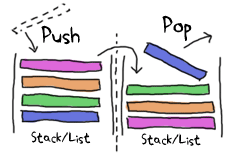
\includegraphics[width=0.4\textwidth]{fifo.png}
\end{figure}
На картинке представлена примерная реализация: два списка (в этом контексте стеки), которые позволяют быстро добавлять элементы в голову и хвост очереди.

Модуль queue содержит несколько функций, которые мысленно можно отнести к трём интерфейсам (или API) различной сложности.
Они называются <<Оригинальный API>>, <<Расширенный API>>, и <<Okasaki API>>:
\\

\begin{minipage}{1.0\linewidth}
    \textbf{Оригинальный API}\\
    Оригинальный API содержит функции, реализующие базовые свойства очереди.
    В их число входят: \ops{\href{http://erldocs.com/R15B/stdlib/queue.html\#new/0}{new/0}} создаёт пустую очередь, \ops{\href{http://erldocs.com/R15B/stdlib/queue.html\#in/2}{in/2}} вставляет новый элемент, \ops{\href{http://erldocs.com/R15B/stdlib/queue.html\#out/1}{out/1}} удаляет элемент. Здесь также есть функции для конвертации очереди в список, для изменения порядка элементов на противоположный, для определения вхождения какого\--либо значения в очередь и т.д.\\
    \\
    \textbf{Расширенный API}\\
    В расширенном API, главным образом, введены средства, придающие структуре гибкость, и позволяющие осуществлять интроспекцию.
    С их помощью можно, например, извлекать головной элемент без его удаления (см. \ops{\href{http://erldocs.com/R15B/stdlib/queue.html\#get/1}{get/1}} или \ops{\href{http://erldocs.com/R15B/stdlib/queue.html\#peek/1}{peek/1}}), просто удалять элементы, не заботясь об их значении (\ops{\href{http://erldocs.com/R15B/stdlib/queue.html\#drop/1}{drop/1}}), и т.д.
    Эти функции нельзя отнести к основам, составляющим концепцию очереди, но всё равно они весьма полезны.\\
    \\
    \textbf{Okasaki API}\\
    Okasaki API немного странный.
    Он взят из книги Chris Okasaki \href{http://books.google.ca/books?id=SxPzSTcTalAC&lpg=PP1&dq=chris\%20okasaki\%20purely\%20functional\%20data\%20structures&pg=PP1\#v=onepage&q=&f=false}{Purely Functional Data Structures}.
    Этот API предоставляет набор операций, похожий на предыдущие два, но некоторые имена функций в нём записываются задом\--наперёд, и в целом этот API весьма своеобразен.
    Если вы не вполне уверены, что вам нужен именно этот API, то лучше с ним не связывайтесь.\\
\end{minipage}

Очереди обычно используют, когда необходимо убедиться, что первый по порядку элемент точно будет обработан первым.
Те примеры, которые я показывал ранее, в качестве аккумуляторов в основном использовали списки, которые мы разворачивали в конце вычислений.
Если вы не можете развернуть сразу весь список, или в аккумулятор приходится часто добавлять новые элементы, то вам скорее всего нужен модуль queue (конечно же, вы сперва должны провести измерения и всё проверить!
Первым делом всё всегда нужно измерять и проверять!)
\section{Окончание краткого обзора}
\label{end-of-the-short-visit}
Вот и закончен наш краткий экскурс в структуры данных Erlang.
Спасибо, что во время путешествия не высовывали руки за пределы транспортного средства.
Есть, конечно же, и другие структуры данных, которые помогают в решении различных задач.
Я осветил лишь те, которые вам пригодятся больше всех, и с которыми, учитывая специфику задач решаемых с помощью  Erlang, вы точно столкнётесь.
Для поиска дополнительных сведений рекомендую обратиться к \href{http://www.erlang.org/doc/apps/stdlib/index.html}{стандартной} и \href{http://www.erlang.org/doc/applications.html}{расширенной} библиотеке.

Вас наверняка порадует, что на этом мы завершаем путешествие в последовательный (sequential) (функциональный) Erlang.
Я знаком со многими людьми, которые начали изучать  Erlang из\--за параллелизма, процессов и всего прочего.
И это неудивительно, ведь Erlang блестяще справляется с задачами именно в этих областях.
К вашим услугам: деревья контроля, развитая система управления ошибками, распределённость и многое другое.
Знаю, что из\--за собственной нетерпеливости я уже касался этих тем, а некоторые читатели уже наверняка о них успели прочитать.

Тем не менее, я посчитал, что перед переходом к параллельному Erlang нужно привыкнуть к его функциональной стороне.
Так нам будет легче продвигаться по материалу и концентрироваться лишь на новых концепциях.
Начинаем!
\begin{figure}[h!]
    \centering
    
\includegraphics[width=0.7\textwidth]{squid-concurrency.png}
\end{figure}
